\documentclass{article}

\usepackage{graphicx}
\usepackage{booktabs}
\usepackage{amsmath}

\usepackage{biblatex}
\addbibresource{resources.bib}

\usepackage{tikz}
\usetikzlibrary{arrows.meta}

\usepackage{pdfpages}

\title{Discontinuous Mode Flyback Transformer Design}
\author{Andrew Meares}
\date{January 2025}

\begin{document}

\maketitle

\section{Introduction}
This paper serves as a guide for discontinuous mode flyback transformer design for small low power isolated DC/DC converters.
Readers are encouraged to familiarize themselves with the workings of flyback converters before delving into this material and the accompanying spreadsheet tool.

\begin{figure}[h]
\centering
\includegraphics[height=4cm]{flyback1.jpg}
\caption{Characteristic flyback converter circuit with transformer.}
\label{fig:flyback_example}
\end{figure}

Flyback converters can operate in two modes: continuous mode and discontinuous mode. Continuous mode occurs when the transformer’s core stores some residual energy at the end of each switching cycle. In contrast, discontinuous mode ensures that all the energy stored in the transformer’s magnetic core is transferred to the load during each switching cycle, leaving the core energy-free before the next cycle begins. This paper focuses on designing transformers specifically for discontinuous mode operation.

Key features of discontinuous mode operation are that it simplifies control and stabilization while reducing reverse recovery losses. These characteristics make discontinuous mode attractive for applications with low to moderate power requirements. However, it also introduces higher peak currents, which can limit the power handling capacity of the transformer and associated components. Continuous mode designs may offer higher efficiency at higher power levels but require additional complexity, such as slope compensation circuits, to manage stability and noise.

This paper assumes the use of the UC3845A or a similar PWM controller, which imposes a maximum duty cycle limitation of 50\%. There is also a comparison between two design variants to illustrate how to gauge if a design is achievable on a particular core size and material.

\section{Design Requirements}
While the PWM controller, such as the UC3845A or a similar IC, plays a critical role in the overall operation, the focus here is specifically on transformer design. Readers should refer to the relevant datasheets for additional circuit application notes. The circuit operates using a peak current mode control methodology.
Two variants of requirements are used to provide some comparisons.

Previous experience and a survey of existing solutions inform 
that this converter will have a relatively low efficiency.
Consider 80\% efficiency a great success and at lower output power, the efficiency 
is in the 70\% to 80\% range.

\begin{table}[h]
    \centering
    \begin{minipage}{0.45\textwidth}
        \centering
        \begin{tabular}{@{} l c @{}}
            \toprule
            Parameter & Value \\
            \midrule
            \( V_{\text{out}} \) & 21 V \\
            \( V_{\text{in}} \) & 19-24 V \\
            \( P_{\text{out}} \) & 2 W \\
            Efficiency Goal & 75 \% \\
            \bottomrule
        \end{tabular}
        \caption{Design I}
        \label{tab:specs1}
    \end{minipage}%
    \hspace{0.05\textwidth} % Adjust horizontal space as needed
    \begin{minipage}{0.45\textwidth}
        \centering
        \begin{tabular}{@{} l c @{}}
            \toprule
            Parameter & Value \\
            \midrule
            \( V_{\text{out}} \) & 8-12 V \\
            \( V_{\text{in}} \) & 19-24 V \\
            \( P_{\text{out}} \) & 8 W \\
            Efficiency Goal & 80 \% \\
            \bottomrule
        \end{tabular}
        \caption{Design II}
        \label{tab:specs2}
    \end{minipage}
\end{table}

\section{Theory}
In order to design this transformer, some theoretical foundation is needed.
One basic assumption that is often overlooked, I will state at the beginning.
\textbf{We start by assuming that the design is achievable.}

\subsection{Faraday's Law of Induction}

The following is adapted from Ulaby \cite[pp. 256--257]{ulaby2007fae}.

\begin{equation}
    \epsilon = - \frac{d \Phi_B}{dt}
    \label{eq:faraday1}
\end{equation}

\emph{The electromotive force around a closed path is equal to the negative of the time rate of change of the magnetic flux enclosed by the path.} \\

For a coil with multiple turns of wire, the relationship becomes:

\begin{equation}
    \epsilon = - N \frac{d \Phi_B}{dt}
    \label{eq:faraday2}
\end{equation}

This is because each wire loop contributes to the total flux linkage, effectively multiplying the induced electromotive force.

\subsection{Definition of Inductance}

\emph{Inductance is the ratio of the change in magnetic flux and the current that generates it \cite[p. 239]{ulaby2007fae}.}

\begin{equation}
    L = \frac{\Phi_B}{I}
    \label{eq:inductance1}
\end{equation}

Combining those two thoughts:

% \epsilon = - \frac{d \Phi_B}{dt} = - \frac{d}{dt} (LI) = -L \frac{dI}{dt}
\begin{equation}
    \epsilon = - \frac{d \Phi_B}{dt} = - \frac{d}{dt} (LI) = -L \frac{dI}{dt}
    \label{eq:inductance2}
\end{equation}

The electromotive force is equal to the negative of the inductance times
the rate of change of the current.  In this application,
the important result is that the voltage across the inductor is equal to the
rate of change of the current times the inductance.

% V_L = L \frac{di}{dt}
\begin{equation}
    V_L = L \frac{di}{dt}
    \label{eq:inductance3}
\end{equation}

Now consider the amount of energy stored in a magnetic field.

\subsection{Definition of Electric Power}
As defined by the International System of Units (SI):
\begin{quote}
"The watt is the power which in one second gives rise to energy of 1 joule." \cite[p. 160]{si2019}
\end{quote}

Apply that to the inductor case and consider ramping to a final current I, in t seconds:

\begin{align}
    P &= \text{"work done per unit time"} = \frac{VQ}{t} = VI \\
    V_L &= L \frac{di}{dt} \\
    P_L &= L \frac{di}{dt} I \\
    E_L &= \int_{0}^{t} P_L \, dt = \int_{0}^{I} L(i) \, di = \frac{1}{2} LI^2
    \label{eq:power2}
\end{align}

\section{Design}

Both designs are shown in parallel, as that yields some interesting 
comparisons.
For a flyback in discontinuous mode, the inductor is charged to a peak
current and then discharged back to zero.  This happens at the switching
frequency.  Therefore, the power stored in the magnetic field is given by:

\begin{equation}
    P = \frac{1}{2} LI^2 f_{\text{sw}}
    \label{eq:power3}
\end{equation}

\emph{Note that the power transferred by the coupled inductor is less than the input power and more than the output power, e.g. the efficiency is always less than 100\%.}

\subsection{Calculate $I_{pk}$}

We can limit our duty cycle of the main switch to 40\% to ensure that we operate always in discontinuous mode.  This is a bit of a shortcut
since the true limitation is that the on time of the main switch plus the
duty cycle of the secondary side rectifier must be less than the switching
period in order for the current to ramp down to zero before the next cycle.
If we assume that the secondary side duty cycle is equal to the primary side,
then if we limit both to less than 50\% with some margin, then we are
operating in the discontinuous mode.

If we use 40\% of each cycle to ramp from 0 to Ipk, then we can
calculate the average current during the entire cycle and use that to find
the peak current required to establish that average input current.

%\begin{figure}[h]
%    \centering
%    \begin{tikzpicture}[scale=1, every node/.style={font=\small}]
%        % Axes
%        \draw[->] (0.5,0) -- (5,0) node[right] {Time};
%        \draw[->] (0.5,0) -- (0.5,2.5) node[above] {Current};
%
%        % Labels for axes
%        \node[below] at (0.8,0) {$t_0$};
%        \node[below] at (4.5,0) {$T_{\text{per}}$};
%        \node[left] at (0.5,2) {$I_{\text{pk}}$};
%        \node[left] at (0.5,0.7) {$I_{\text{avg}}$};
%
%        % Primary side triangle (Ton)
%        \fill[blue,opacity=0.3] (0.8,0) -- (2.8,0) -- (2.8,2) -- cycle; % Blue triangle
%        \draw[thick,blue] (0.8,0) -- (2.8,2);
%        \draw[thick,blue] (2.8,2) -- (2.8,0);
%        % Mark peak currents
%        \draw[dashed] (2.8,2) -- (0.5,2);
%        % Draw Iavg
%        \draw[dashed] (0.5,0.7) -- (4.5,0.7);
%
%        % Duty cycle indication
%        \draw[<->,blue] (0.9,-0.2) -- (2.8,-0.2) node[midway,below] {$t_{\text{on}}$};
%    \end{tikzpicture}
%    \caption{Flyback Primary Current Waveform in Discontinuous Mode}
%    \label{fig:flyback1}
%\end{figure}

\begin{figure}[h]
    \centering
    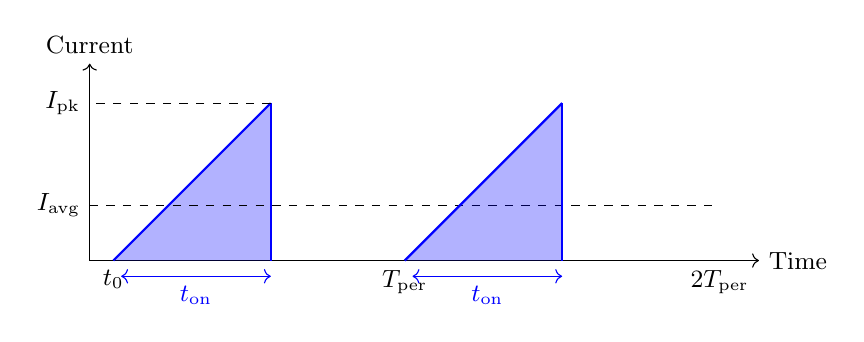
\begin{tikzpicture}[scale=1, every node/.style={font=\small}]
        % Axes
        \draw[->] (0.5,0) -- (9,0) node[right] {Time};
        \draw[->] (0.5,0) -- (0.5,2.5) node[above] {Current};

        % Labels for axes
        \node[below] at (0.8,0) {$t_0$};
        \node[below] at (4.5,0) {$T_{\text{per}}$};
        \node[below] at (8.5,0) {$2T_{\text{per}}$};
        \node[left] at (0.5,2) {$I_{\text{pk}}$};
        \node[left] at (0.5,0.7) {$I_{\text{avg}}$};

        % Primary side triangle (Ton) - First Period
        \fill[blue,opacity=0.3] (0.8,0) -- (2.8,0) -- (2.8,2) -- cycle; % Blue triangle
        \draw[thick,blue] (0.8,0) -- (2.8,2);
        \draw[thick,blue] (2.8,2) -- (2.8,0);
        
        % First Period: Mark peak currents and Iavg
        \draw[dashed] (2.8,2) -- (0.5,2);
        \draw[dashed] (0.5,0.7) -- (8.5,0.7);

        % Duty cycle indication - First Period
        \draw[<->,blue] (0.9,-0.2) -- (2.8,-0.2) node[midway,below] {$t_{\text{on}}$};

        % Primary side triangle (Ton) - Second Period
        \fill[blue,opacity=0.3] (4.5,0) -- (6.5,0) -- (6.5,2) -- cycle; % Blue triangle
        \draw[thick,blue] (4.5,0) -- (6.5,2);
        \draw[thick,blue] (6.5,2) -- (6.5,0);

        % Duty cycle indication - Second Period
        \draw[<->,blue] (4.6,-0.2) -- (6.5,-0.2) node[midway,below] {$t_{\text{on}}$};
    \end{tikzpicture}
    \caption{Flyback Primary Current Waveform in Discontinuous Mode}
    \label{fig:flyback1}
\end{figure}


\noindent % Ensures the minipages start at the leftmost part of the page.
\begin{minipage}[t]{0.45\linewidth} % 0.5\linewidth means this minipage will take up half the width of the page.
    \begin{itemize}
        \renewcommand\labelitemi{} % Remove the default bullet
        \item \textbf{Design I}
        \item \( V_{\text{in}} = 21\, \text{V} \)
        \item \( P_{\text{out}} = 2\, \text{W} \)
        \item \( D_{\text{max}} = 40\% \)
        \item Efficiency Goal = \( 75\% \)
        \item \( P_{\text{i}} = \frac{P_{\text{out}}}{\eta} = \frac{2}{0.75} = 2.7\, \text{W} \)
        \item \( I_{\text{avg}} = \frac{P_{\text{i}}}{V_{\text{in}}} = \frac{2.7\, \text{W}}{21\, \text{V}} = 129\, \text{mA} \)
        \item \( I_{\text{pk}} = 2\left(\frac{I_{\text{avg}}}{D_{\text{max}}}\right) = 643\, \text{mA} \)
    \end{itemize}
\end{minipage}%
\hfill % This fills the space between the two minipages. Since each is set to half the width, this will be minimal.
\begin{minipage}[t]{0.45\linewidth}
    \begin{itemize}
        \renewcommand\labelitemi{} % Remove the default bullet
        \item \textbf{Design II}
        \item \( V_{\text{in}} = 21\, \text{V} \)
        \item \( P_{\text{out}} = 8\, \text{W} \)
        \item \( D_{\text{max}} = 40\% \)
        \item Efficiency Goal = \( 80\% \)
        \item \( P_{\text{i}} = \frac{P_{\text{out}}}{\eta} = \frac{8}{0.8} = 10\, \text{W} \)
        \item \( I_{\text{avg}} = \frac{P_{\text{i}}}{V_{\text{in}}} = \frac{10\, \text{W}}{21\, \text{V}} = 476\, \text{mA} \)
        \item \( I_{\text{pk}} = 2\left(\frac{I_{\text{avg}}}{D_{\text{max}}}\right) = 2.38\, \text{A} \)
    \end{itemize}
\end{minipage} \\

The peak current calculated above is what is required to generate
the average input current required to power the converter under full load.
Note that this does not depend on switching frequency.

\subsection{Choose Inductance and Switching Frequency}

In order to figure out what our primary winding inductance should be, we 
must choose a switching frequency.  The inductance we calculate is sometimes
called the minimum inductance but I like to think of it as a nominal value
and adjust the peak current set point and frequency in the prototype to
obtain the desired power output.

\begin{equation}
    P = \frac{1}{2} LI^2 f_{\text{sw}} \quad \text{and} \quad L = \frac{2P}{I^2 f_{\text{sw}}}
    \label{eq:inductance4}
\end{equation}

Choosing the nominal inductance based
on a switching frequency and a peak current set point is easy.  The problem is
that the inductance found does not always mesh well with our selection of cores,
bobbins, and magnet wire.

A discontinuous mode design does not have a “DC” component of current in the magnetic
component.  That means that the current flowing is triangle wave pulses with harmonic
content starting at the switching frequency.  The skin effect is an important concept.
A description directly lifted from the Wikipedia page is stated below: \\

\emph{Skin effect is the tendency of an alternating electric current (AC) to become
distributed within a conductor such that the current density is largest near the
surface of the conductor, and decreases with greater depths in the conductor.} \\

In order to keep things simple, we will not investigate other effects such as proximity
effect which add another layer of complexity and can be significant.  The skin effect
alone can raise the effective resistance of a winding significantly.  All of our
current is “AC” in a discontinuous mode design.  Therefore our magnet wire’s diameter
should be no more than twice the skin depth at the switching frequency we are operating
at.

Another constraint is that all of the windings must fit within the chosen core and 
bobbin’s window area.  The utilization factor is the ratio of the used bobbin window
area to the total bobbin window area and is never 100\%.  You might often see the total
window area metric be with respect to the core window area.  We are taking the bobbin
into account here.

Let us initially consider a switching frequency of 160kHz initially for both designs.
This is because a 4.99kOhm resistor and a 1nF capacitor result in approximately this
frequency when used in the UC3845A oscillator circuit.  After we choose cores, we will
reconsider our switching frequency and see if our design is optimal. \\

\noindent % This ensures that the minipages start at the leftmost part of the page.
\begin{minipage}[t]{0.45\linewidth} % 0.5\linewidth means this minipage will take up half the width of the page.
    \begin{itemize}
        \renewcommand\labelitemi{} % Remove the default bullet
        \item \textbf{Design I}
        \item $L = \frac{2P}{I^2 f_{\text{sw}}} = \frac{2(2.7\, \text{W})}{(0.643\, \text{A})^2 \times 160\, \text{kHz}}$ \\
        \item $L = 82\, \mu\text{H}$
    \end{itemize}
\end{minipage}%
\hfill % This fills the space between the two minipages. Since each is set to half the width, this will be minimal.
\begin{minipage}[t]{0.45\linewidth}
    \begin{itemize}
        \renewcommand\labelitemi{} % Remove the default bullet
        \item \textbf{Design II}
        \item $L = \frac{2P}{I^2 f_{\text{sw}}} = \frac{2(10\, \text{W})}{(2.38\, \text{A})^2 \times 160\, \text{kHz}}$ \\
        \item $L = 22\, \mu\text{H}$
    \end{itemize}
\end{minipage} \\

As stated previously, these inductance values calculated are “minimum” values because any
less inductance would store too little energy per cycle to maintain the maximum output
power.  Still, consider these “nominal” because in truth you can simply adjust
frequency, peak current set point, or maximum duty cycle to compensate for a small
deficiency in inductance.  Another way to think about this is that we are putting a
size on the cores here.  The inductances we found are secondary.  Increasing the peak
current set point increases the maximum flux density applied to the core and other
parameters have similar impacts.

\subsection{An Aside on Volt-Seconds}

The total duty cycle, Tper, is made up of 3 parts:
\begin{itemize}
    \item Ton, the time the main transistor is on.
    \item Treset, the time the energy is transferred to the load
    \item Textra, the time left over.
    \item Tper = Ton + Treset + Textra
\end{itemize}

With a duty cycle maximum of 40\%, a switching frequency of 160kHz, and an input voltage
of 21V, during Ton, we apply $21V(0.4)(T_{\text{per}}) = 52.5\, V\mu s$ , read 52.5 
volt-microseconds, to the core during every switching cycle’s on time.

A simple relationship to always keep in mind follows:

\begin{equation}
    V_{\text{in}} T_{\text{on}} = V_{\text{out}} T_{\text{reset}}
    \label{eq:voltseconds1}
\end{equation}

One way to think of the losses in the circuit is that the main transistor, the shunt
resistor, the rectifier diode, and the winding’s impedance, all take away from the
applied volt seconds per cycle.  We are not going to factor them into our calculations
other than as part of the “total efficiency” of the converter.

\subsubsection{More about Duty Cycle}

The secondary duty cycle, $T_{\text{reset}}$, corresponds to the reset time during which the energy stored in the magnetic field is transferred to the load via the secondary-side rectifier diode. During this period, the voltage across the secondary-side inductance, $V_{\text{reset}}$, is maintained by the output capacitor, which stabilizes the output at the desired voltage level.

%Consider the secondary duty cycle, $T_{\text{reset}}$,   During the reset time, the
%energy stored in the magnetic field is transferred to the load through the secondary
%side rectifier diode.  During this time, the voltage across the secondary side
%inductance, Vreset, is provided by the output capacitor which clamps the output at
%the current output voltage.

This is reflected back to the primary at 
$V_{\text{reset}} = V_{\text{out}} \times \frac{1}{N_{\text{PS}}}$
, where $N_{\text{PS}}$ is the primary side to secondary side turns ratio.  So the duty 
cycle of the secondary side is
$N_{\text{PS}} \times \frac{V_i}{V_o}$
times the primary side duty cycle.  My takeaway from this is that if 
$N_{\text{PS}} \leq 1$
then the $T_{\text{on}} + T_{\text{reset}}$
will always be less than $T_{\text{per}}$ 
and discontinuous mode operation is certain if the maximum duty cycle is less than 50\%.  On an offline flyback with a high
voltage input and low voltage output, the turns ratio will be higher.  This often
results in the converter being designed to operate in continuous mode conduction
through some of its operating range.

\section{Pick a Core}

The energy stored in the flyback converter is in the magnetic field of the coupled
inductor that is used to transfer energy to the load.  The core of this inductor
is usually gapped to increase its energy storage capability.  Some designs use
distributed gap material instead.  We need to create the minimum inductance with
also the ability to withstand the applied maximum volt-seconds without saturating
the core.

The energy stored in a magnetic field of an inductor is:
$E = \frac{1}{2} LI^2$

For a generic core, $L = \frac{\mu N^2 A}{l}$.  This result comes fairly directly
from Faraday’s law of induction applied to a solenoid.

\begin{equation}
    L = \frac{N \Phi_B}{I} = \frac{\mu_r \mu_0 N I}{l_{\text{eff}}} \times \frac{N}{I} = \frac{N^2 \mu_0 \mu_r a}{l_{\text{eff}}}
    \label{eq:inductance5}
\end{equation}

We tend to model magnetic structures as their far simpler ideal counterparts.
By using the term, $l_{\text{eff}}$, or effective magnetic path length, we can
accommodate for the various shapes of cores using this one corrective term.
I usually just let the magnetics manufacturers figure out $l_{\text{eff}}$ for me.

The definition of I is per turn, so the addition of extra loops multiplies the
applied current through the amperian loop.  So if the rate of change of the current
is 1A/s and the number of turns is 10, then you get 10A/s through the amperian loop.
Note the cross sectional area, \textbf{a}, is introduced because the B field is the density
per unit area and the flux is equal to B times \textbf{a}.

In terms of applied magnetic field, H, and resulting flux density, B, the energy
stored in the gap is derived below:

\begin{align}
    E_L &= \int_{0}^{t} P_L \, dt = \int_{0}^{I} L(i) \, di = \frac{1}{2} LI^2 \\
    E_L &= \frac{1}{2} LI^2 = \frac{1}{2} \frac{N^2 \mu_r \mu_0 a}{l} I^2
    \label{eq:energy1}
\end{align}

Since $H = \frac{N I}{L}$

\begin{align}
E = \frac{1}{2} L I^2 = \frac{1}{2} \mu_r \mu_0 H^2 = \frac{1}{2} B H
\label{eq:energy2}
\end{align}
The above result is in Joules per cubic meter (\(\text{J}/\text{m}^3\)), based on the following units: \(B\) is in Weber per square meter (\(\text{Wb}/\text{m}^2\)) and \(H\) is in amperes per meter (\(\text{A}/\text{m}\)).

Let us make another assumption, that the relative permeability of the core material is much greater than that of air (\(\mu_{r,\text{air}} = 1\)) and the gap is small in length compared to the mean magnetic path length.
The integral form of Gauss’s law for magnetism states that the surface integral over an enclosed surface of \( \vec{B} \cdot d\vec{A} \) is equal to zero.
This means that the sum of all the fluxes at the gap interface is zero, and the flux in the core is equal to the flux in the gap minus the flux that escapes (fringing flux).
Note that since the flux density is multiplied by the relative permeability in the core, this means the applied magnetic field, \(H\), is far less in the core than in the gap.
Therefore, as long as the mean path length divided by the relative permeability of the core is smaller in magnitude than the effective gap length, more of the energy is stored in the gap than in the core.

The fringing flux can be a quite significant loss factor or nearly insignificant.  It all depends on how you build it.  We are going to generally ignore fringing flux but a few tips will help:
\begin{itemize}
    \item Gapping the center leg of the EE core set helps contain the fringing flux.
    \item Gapping all three legs of the EE core set will result in poorer containment and performance but it generally still works.
    \item Using a few layers of thin tape on all three legs is much easier to do in the lab than to carefully file down the center leg.
    \item The gap interface and the core to core interfaces are extremely important.  For zero gap, two core surfaces must be precisely smooth and clean to mate optimally.  Even a small imperfection can have an outsized effect due to the mismatch in effective permeability.
    \item For a gapped core, chips in the outer edges of the gapped area from tools will increase the fringing flux.
\end{itemize}

\section{Gap Volume and Energy Storage}
So let's figure out the volume of the gap required to store our energy quantum!
If the input power is \(2.7 \, \text{W}\) and that is delivered to the load in \(160\text{k}\) packets of energy per second. To store \(16.9 \, \mu\text{J}\), we need to find an appropriate gapped core.

\begin{align}
\text{Energy per packet} = \frac{\text{Input Power}}{\text{Packets per second}} = \frac{2.7 \, \text{W}}{160 \, \text{kHz}} = 16.9 \, \mu\text{J}
\end{align}

Consider a small EE core set, \(E13/7/4\) from Ferroxcube. This core’s center leg is \(3.7 \, \text{mm}\) on each side. Due to its availability, we will consider \(3C94\) material. Pick a maximum \(B\) field level that provides a sufficient margin to the saturation level for the material. Ferroxcube specifies a defined level of saturation for \(3C94\) material at \(10 \, \text{kHz}/100^\circ \text{C}\) of \(380 \, \text{mT}\). Provide a wide margin as the saturation level can vary greatly over frequency, temperature, and definition. We are going to choose \(180 \, \text{mT}\).

\begin{align}
B &= \mu_r \mu_0 H \\
E \, (\text{Joules}) &= \frac{1}{2} B H A_e L_g = \frac{1}{2} B^2 \frac{1}{\mu_r \mu_0} A_e L_g \\
\frac{1}{2} L I^2 &= \frac{1}{2} B^2 \frac{1}{\mu_r \mu_0} A_e L_g \\
A_e L_g &= \frac{L I^2 \mu_r \mu_0}{B_\text{pk}^2}
\end{align}

\noindent % This ensures that the minipages start at the leftmost part of the page.
\begin{minipage}[t]{0.45\linewidth}
    \textbf{Design I}
    \begin{align*}
        A_e &= (3.7 \, \text{mm})^2 = 13.7 \, \text{mm}^2 \\
        A_e L_g &= \frac{L I^2 \mu_r \mu_0}{B_\text{pk}^2} \\
        A_e L_g &= \frac{82 \, \mu\text{H} \, (0.643 \, \text{A})^2 \, (1) \, \mu_0}{(180 \, \text{mT})^2} = 1.3 \, \text{mm}^3
    \end{align*}
    Revising the number with the slightly lower \(A_\text{effective} = 12.4 \, \text{mm}^2\) from the core’s datasheet yields:
    \begin{align*}
    L_g = \frac{1.3 \, \text{mm}^3}{12.4 \, \text{mm}^2} = 0.1 \, \text{mm}
    \end{align*}
\end{minipage}
\begin{minipage}[t]{0.45\linewidth}
    \textbf{Design II}
    \begin{align*}
    A_e &= (3.7 \, \text{mm})^2 = 13.7 \, \text{mm}^2 \\
    A_e L_g &= \frac{L I^2 \mu_r \mu_0}{B_\text{pk}^2} \\
    A_e L_g &= \frac{22 \, \mu\text{H} \, (2.8 \, \text{A})^2 \, (1) \, \mu_0}{(180 \, \text{mT})^2} = 6.7 \, \text{mm}^3
    \end{align*}
    Revising the number with the slightly lower \(A_\text{effective} = 12.4 \, \text{mm}^2\) from the core’s datasheet yields:
    \begin{align*}
    L_g = \frac{6.7 \, \text{mm}^3}{12.4 \, \text{mm}^2} = 0.54 \, \text{mm}
    \end{align*}
\end{minipage} \\

Design 1 has a small gap of only \(3.9 \, \text{mil}\) or \(0.1 \, \text{mm}\).
Design 2 has a larger gap of \(21.2 \, \text{mil}\) or \(0.54 \, \text{mm}\).
I am skeptical that Design 2 will fit on the 13/7/4 core set.

\section{What is \(A_L\)?}
\(A_L\) is usually reported in \(\text{nH/Turn}^2\). Remember 
\[
L = \frac{N^2 \mu_r \mu_0 a}{l}?
\]
Extract the \(N^2\) term and you have the permeance, or inductance per turn squared coefficient.

\section{Estimate \(A_L\) for the Core}
Ferroxcube was nice enough to provide measured AL values for different gaps.  There are multiple approaches possible here.  Based on the linear relationship assumed between B and H, the permeance of a gapped core can be estimated using the formula below:
\begin{align}
A_L &= \frac{\mu_0 a}{l_\text{eff} + \frac{l_g}{\mu_r}}
\end{align} \\

\begin{minipage}[t]{0.45\linewidth}
    \textbf{Design I}
    \begin{align*}
        \mu_r &= 1525 \\
        l_e &= 29.7 \, \text{mm} \\
        a_e &= 12.4 \, \text{mm}^2 \\
        A_L &= \frac{\mu_0 a}{l_g + \frac{l_\text{eff}}{\mu_r}} \\
        A_L &= \frac{\mu_0 \cdot 12.4 \, \text{mm}^2}{0.1 \, \text{mm} + \frac{29.7 \, \text{mm}}{1525}} = 126 \, \text{nH}/N^2
    \end{align*}
    The ungapped \(A_L\) value for comparison is:
    \begin{align*}
    A_L &= \frac{\mu_r\mu_0 a}{l_\text{eff}} \\
    A_L &= \frac{1525 \cdot \mu_0 \cdot 12.4 \, \text{mm}^2}{29.7 \, \text{mm}} = 800 \, \text{nH}/N^2
    \end{align*}
    The ungapped value agrees with the datasheet as I hoped, but the gapped value given in the datasheet is \(A_L = 160 \, \text{nH}/N^2\). Perhaps they measured it or are accounting for more variables than our simple estimate. We will use the datasheet numbers wherever we can.
\end{minipage}
\begin{minipage}[t]{0.45\linewidth}
    \textbf{Design II}
    \begin{align*}
    \mu_r &= 1525 \\
    l_e &= 29.7 \, \text{mm} \\
    a_e &= 12.4 \, \text{mm}^2 \\
    A_L &= \frac{\mu_0 a}{l_g + \frac{l_\text{eff}}{\mu_r}} \\
    A_L &= \frac{\mu_0 \cdot 12.4 \, \text{mm}^2}{0.49 \, \text{mm} + \frac{29.7 \, \text{mm}}{1525}} = 2 \, \text{nH}/N^2
    \end{align*}
    Looking at the datasheet, Ferroxcube specifies that for a \(320 \, \mu\text{m}\) gap, the \(A_L\) value is \(63 \, \text{nH}/N^2\). As this is their largest specified gap, I am continuing to suspect this core set is too small for the required power level. 
    
    One might consider the value for a relatively large gap competently estimated by the following simplification:
    \begin{align*}
    A_L = \frac{\mu_0 a}{l_g} = 29 \, \text{nH}/N^2
    \end{align*}
\end{minipage}

\section{Calculate NP, NS, and NB}
\begin{minipage}[t]{0.45\linewidth}
    \textbf{Design I}
    \begin{align*}
    A_L &= 160 \, \text{nH}/N^2 \\
    L &= A_L N^2 \\
    N &= \sqrt{\frac{L}{A_L}} \\
    N_P &= \sqrt{\frac{82 \, \mu\text{H}}{160 \, \text{nH}/N^2}} = 23 \, \text{Turns}
    \end{align*}
\end{minipage}
\begin{minipage}[t]{0.45\linewidth}
    \textbf{Design II}
    \begin{align*}
    A_L &= 29 \, \text{nH}/N^2 \\
    N_P &= \sqrt{\frac{22 \, \mu\text{H}}{29 \, \text{nH}/N^2}} = 28 \, \text{Turns}
    \end{align*}
\end{minipage} \\

The turns ratio between the primary and secondary affects the voltage stress on the primary switch. One estimate for the primary switch voltage rating is given by Pressman below and recommends at least a 30\% margin. It seems that \(100 \, \text{V}\) FETs are highly available in various packages with optimized performance. In order to capitalize on increased performance with lower voltage FETs, the next popular voltage rating down is \(60 \, \text{V}\), which might be worth considering.

\begin{align}
V_\text{DSS} \geq 1.3 \times \left( V_\text{in} + \frac{1}{N_\text{PS}} V_o \right)
\end{align}

There is a relatively simple relationship between the secondary output voltage and the bias winding output voltage.  Disregarding diode forward voltages and loading and a bunch of other stuff:

\begin{align}
V_\text{bias} = \frac{N_B}{N_S} V_\text{out}
\end{align} \\

\begin{minipage}[t]{0.45\linewidth}
    \textbf{Design I}
    \begin{align*}
    V_\text{DSS} \geq 1.3 \times \left( 21 \, \text{V} + \frac{1}{N_\text{PS}} 21 \, \text{V} \right)
    \end{align*}
    Since \(N_P\) is 23 turns, I like choosing \(N_S\) as 21 turns so that \(N_B\) is 12 turns, or 1 turn per volt.
    \begin{align*}
    N_\text{PS} &= \frac{21}{23} = 0.9 \\
    V_\text{DSS} &\geq 1.3 \times \left( 21 + \frac{23}{21} \cdot 21 \right) \\
    V_\text{DSS} &\geq 57.2 \, \text{V}
    \end{align*}
\end{minipage}
\begin{minipage}[t]{0.45\linewidth}
    \textbf{Design II}
    \begin{align*}
    N_\text{PS} &= \frac{18}{28} = 0.64 \\
    V_\text{DSS} &\geq 1.3 \times \left( 21 + \frac{28}{18} \cdot 9 \right) \\
    V_\text{DSS} &\geq 45.5 \, \text{V}
    \end{align*}
\end{minipage} \\

From the bobbin drawing in the Ferroxcube datasheet for the CPH-E13/7/4-1S-6P coil former, we get a window area of 11.6mm2.  For this thought experiment we will consider the total number of turns required to make the primary winding, secondary winding, and bias winding.  We will consider using a single wire gauge at first and a fill factor of 50\%.  The fill factor is to account for wires not packing perfectly and lost window area taken up by tape and air.  Packing same-size round wires has an efficiency of 90.7\% at best \cite{circle_packing}. \\

\begin{minipage}[t]{0.45\linewidth}
    \textbf{Design I}
    \begin{align*}
    N_\text{total} &= N_P + N_S + N_B \\
    N_\text{total} &= 23 + 21 + 12 = 56 \\
    A_\text{wire} &= \frac{0.75 \, A_\text{window}}{N_\text{total}} \\
    A_\text{wire} &= \frac{0.75 \cdot 11.6 \, \text{mm}^2}{56} = 0.155 \, \text{mm}^2 \\
    A_\text{wire} &= \pi r^2 \\ 
    D_\text{wire} &= 2\sqrt{\frac{A}{\pi}} = 0.445 \, \text{mm}
    \end{align*}
    In imperial units, \(D_\text{wire} = 17.5 \, \text{mil}\), or approximately 26 AWG single build magnet wire.
\end{minipage}
\begin{minipage}[t]{0.45\linewidth}
    \textbf{Design II}
    \begin{align*}
    N_\text{total} &= N_P + N_S + N_B \\
    N_\text{total} &= 28 + 18 + 24 = 70 \\
    A_\text{wire} &= \frac{0.75 \, A_\text{window}}{N_\text{total}} \\
    A_\text{wire} &= \frac{0.75 \cdot 11.6 \, \text{mm}^2}{70} = 0.124 \, \text{mm}^2 \\
    D_\text{wire} &= 2\sqrt{\frac{0.124 \, \text{mm}^2}{\pi}} = 0.398 \, \text{mm}
    \end{align*}
    In imperial units, \(D_\text{wire} = 15.7 \, \text{mil}\), or approximately 27 AWG single build magnet wire.
\end{minipage} \\

Note that design 2 requires more power but also only has room for slightly smaller magnet wire.  This is not a good sign.

\section{Consider the Skin Effect}
We should consider skin effect at our switching frequency of 160kHz.
Skin effect at below microwave frequencies for copper is estimated by the following equation taken from Wikipedia:
\begin{align}
\delta = \sqrt{\frac{2 \rho}{2 \pi f \mu_r \mu_0}}
\end{align}

For copper conductors:
\begin{itemize}
    \item \(\rho = 1.69 \, \mu\Omega\cdot\text{cm}\)
    \item \(\mu_r = 0.999994\)
\end{itemize}

Here is a quick breakdown of the approximate largest diameter wire gauge by frequency:

% Table
%\begin{table}[h]
    \begin{center}
    \begin{tabular}{|c|c|c|c|}
        \hline
        \textbf{Freq. (kHz)} & \textbf{Skin Depth (mm)} & \textbf{Wire Dia. (inches)} & \textbf{Wire AWG} \\ \hline
        50  & 0.293 & 0.023 & 23 \\ \hline
        60  & 0.267 & 0.021 & 24 \\ \hline
        70  & 0.247 & 0.019 & 25 \\ \hline
        80  & 0.231 & 0.018 & 26 \\ \hline
        90  & 0.218 & 0.017 & 26 \\ \hline
        100 & 0.207 & 0.016 & 27 \\ \hline
        110 & 0.197 & 0.016 & 27 \\ \hline
        120 & 0.189 & 0.015 & 27 \\ \hline
        130 & 0.181 & 0.014 & 28 \\ \hline
        140 & 0.175 & 0.014 & 28 \\ \hline
        150 & 0.169 & 0.013 & 29 \\ \hline
        160 & 0.164 & 0.013 & 29 \\ \hline
        170 & 0.159 & 0.012 & 29 \\ \hline
        180 & 0.154 & 0.012 & 29 \\ \hline
    \end{tabular}
    \end{center}
%\caption{Skin Depths at Various Frequencies}
%\label{tab:skin_depths}
%\end{table}

The effect of skin depth is telling us that we are wasting copper if we use larger than 29 AWG magnet wire in making our flyback transformer.
This creates an interesting optimization problem.  The choice of inductance is directly proportional to frequency as seen above but we are limited by window area and skin depth in choosing our wire gauge.
Consider the average input current and the estimated length of the primary winding to estimate the primary side winding resistive losses.  The average turn length is given by the bobbin datasheet.  We are going to consider 30 AWG wire.  The datasheet for the magnet wire specifies 103.7 ohms per 1000 ft of wire.

\begin{minipage}[t]{0.45\linewidth}
    \textbf{Design I}
    \begin{align*}
    L_{\text{turn}} &= 24 \, \text{mm} \\
    N_P &= 23 \\
    l_{\text{pri}} &= N_P \cdot L_{\text{turn,avg}} = 552 \, \text{mm} \\
    R_{\text{pri}} &= 552 \, \text{mm} \left(\frac{103.7 \, \Omega}{1000 \, \text{ft}}\right) \left(\frac{1 \, \text{ft}}{304.8 \, \text{mm}}\right) \\
    R_{\text{pri}} &= 0.188 \, \Omega \\
    I_{\text{avg}} &= \frac{P_i}{V_i} = \frac{2.7 \, \text{W}}{21 \, \text{V}} = 129 \, \text{mA}
    \end{align*}
    \emph{Note this is not RMS so we are a bit off.}
    \begin{align*}
    P_{\text{pri}} = (0.129 \, \text{A})^2 \cdot 0.188 \, \Omega = 3.2 \, \text{mW}
    \end{align*}
    For simplicity assume all the windings have the same losses, totaling still less than 10mW.
\end{minipage}
\begin{minipage}[t]{0.45\linewidth}
    \textbf{Design II}
    \begin{align*}
    L_{\text{turn}} &= 24 \, \text{mm} \\
    N_P &= 28 \\
    l_{\text{pri}} &= N_P \cdot L_{\text{turn,avg}} = 672 \, \text{mm} \\
    R_{\text{pri}} &= 672 \, \text{mm} \left(\frac{103.7 \, \Omega}{1000 \, \text{ft}}\right) \left(\frac{1 \, \text{ft}}{304.8 \, \text{mm}}\right) \\
    R_{\text{pri}} &= 0.229 \, \Omega 
    \end{align*}
    Lets assume the secondary with a fewer turns and less than half the voltage has 1.11 amps average (10W at 9V).
    \begin{align*}
    P_{\text{pri}} &= (0.476 \, \text{A})^2 \cdot 0.229 \, \Omega = 52 \, \text{mW} \\
    \end{align*}
    The Cu losses seem significant in this design and the gap is too large for my comfort but it almost still seems possible to fit this design on this core.
\end{minipage}

\section{Optimization of Switching Frequency to Skin Effect}

It turned out previously that skin effect was approximately proportional to the inverse square root of the switching frequency.  Delivered power was proportional to switching frequency and inductance.  There is a tradeoff between switching frequency, bobbin utilization, and winding resistance.

At this point a spreadsheet approach is required.  The definitions of the various parameters, variables, and results are below:

\begin{itemize}
    \item $F_s$, switching frequency
    \item $\rho$, resistivity of copper
    \item $\mu_0$, permeability of free space
    \item $\mu_r (\text{Cu})$, permeability of copper
    \item $\delta$, skin depth at $F_s$ in inches
    \item $W_\text{sd}$, twice the skin depth for picking the wire diameter
    \item $W_\text{awg}$, chosen wire gauge based on bare copper magnet wire diameters
    \item $W_\text{d}$, actual wire diameter of single build copper magnet wire
    \item $R_\text{wire1k}$, resistance of wire for 1000 ft length
    \item $V_\text{in}$, input voltage
    \item $V_\text{o1}$, output voltage 1 (main output)
    \item $V_\text{o2}$, bias output voltage
    \item $P_\text{out}$, output power
    \item $D_\text{max}$, maximum duty cycle
    \item $\eta$, efficiency guess
    \item $P_\text{in}$, input power
    \item $I_\text{in}$, input current average
    \item $I_\text{pk}$, peak switch current set point
    \item $L$, calculated minimum or nominal inductance
    \item $A_\text{e}$, effective cross-sectional area of the core
    \item $B_\text{max}$, chosen maximum flux excursion
    \item $L_\text{g}$, calculated length of the gap in meters
    \item $L_\text{e}$, effective magnetic path length of the core, meters
    \item $\mu_r (\text{core})$, relative permeability of the core
    \item $A_L$, calculated permeance value
    \item $N_\text{ps}$, turns ratio from primary to secondary
    \item $N_\text{p}$, number of primary turns
    \item $N_\text{s}$, number of secondary turns
    \item $N_\text{b}$, number of bias turns
    \item $L_\text{avg,turn}$, average turn length for the bobbin
    \item $A_\text{window}$, window area for the bobbin
    \item $W_\text{window}$, width of the window for the bobbin
    \item $R_\text{p}$, resistance of the primary winding
    \item $R_\text{s}$, resistance of the secondary winding ($V_\text{o1}$)
    \item $R_\text{b}$, resistance of the bias winding ($V_\text{o2}$)
    \item $W_\text{area}$, amount of copper area used
    \item $FF$, fill factor of the bobbin window
\end{itemize}

The basic approach to the optimization is to pick a number of reasonable switching frequencies and wire diameters.  We are taking into account skin effect, so the optimal wire gauge is chosen as the closest to twice the skin depth at the chosen switching frequency.  The configuration that uses a good proportion of the bobbin and minimizes winding resistance is more optimal than a design that does not.

% Insert spreadsheet

The conclusion for the optimization of Design I is that a switching frequency of 120kHz to 140kHz leads to more bobbin utilization and lower resistive losses.  At 100kHz the bobbin utilization was over unity, so that was not a practical design.  Our initial choice of 160kHz was not a terrible one.

% Insert spreadsheet

The conclusion is that a slightly higher switching frequency than Design I is better for Design II and that the design is probably going to get pretty warm at full power but might still be practical.

\section{Quick Notes from the Bench}
I constructed approximations of both Design I and Design II on the bench.  Design I performed well.  Design II did not perform well.  I was able to get about 6W out of Design II but it was very inefficient and did not run smoothly.  I won’t go into details, but I suspect that my gapped core is leaking too much flux.  The total efficiency I obtained was 70\% at 6W output.  It is possible to improve things but I think the better move would be to change Design II to the next size up core set.  I had always suspected this would be the case but I wanted to push the E13 core to the max and see where in the calculations you would find that the design is impractical.
Furthermore, after constructing variants of Design I for different bobbin utilization factors, I found that less than 50\% was far more practical to wind and seemed to be more efficient even though there was often space showing in the window.  This is possibly due to proximity effect as the lower utilization designs have fewer layers as well.

\section{Extra Thoughts on Design I}
For core loss, we can see on the datasheet that 200mT delta B-field at 100kHz (bipolar? sinusoidal?), yields about 0.18W loss per core set.  For a 2.5W input and 80\% efficiency, that would be 7\% of my total power.  That is all pretty hand-wavey since we are applying a unipolar 160mT field at 150kHz, but it is a number to think about.  Perhaps what this is telling me, is that the losses will be greater at higher frequency and higher flux excursion (from zero).  Getting a better number here requires delving into the magnetic material and supplied graphs and equations from your magnetics manufacturer.

For copper loss, we have two sets of 26 turns of 31 AWG wire around a 3.7mm square post.  The primary winding has an average current of 156mA.  Lets just make up a correction factor instead of trying to figure out the real length of the wire.  Say the correction factor is 1.5.

\begin{align*}
L_{\text{pri,wire}} = 26 \cdot (3.7) \cdot (4) \cdot 1.5 \cdot \frac{1}{25.4} = 22 \, \text{inches}
\end{align*}

31 AWG is 131 ohms per 1000 ft.  That gives 0.24 ohms for primary resistance at DC.  Assume the secondary is the same.  The losses are pretty low at <10mW each winding.  Note this quick estimate is based on average current, not RMS.  A random web page skin effect calculator reported that the skin depth for copper at 150kHz is 6mil, which means that skin effect will tend not to increase our winding effective resistance much as our wire radius is only about 4.5 mils.

This is all concluding that Design I’s core is a bit larger than it needs to be.  That said, it is pretty small for a core and I can’t wind much smaller.  Design I is aided by the fact that the voltage is relatively high on both input and output which means I2R losses are diminished.  A secondary of 5V might have 4 times the current and 16 times the copper losses, which would put it in contention with with the core losses.

\section{Conclusion}

The spreadsheet calculator can be used to design flyback transformers using the above method quickly.  The various parameters can all be sourced from the manufacturers core and bobbin datasheets.

\appendix
\section{Datasheet Reference}
The following datasheets are provided for reference:

%\includepdf[pages=1]{uc3845a.pdf}
\includepdf[pages=-]{E13_7_4.pdf}

\printbibliography

\end{document}
